\chapter{Virtual Machine and Programming Language}
\label{chapter:virtual_machine_and_programming_language}

The SALS AI is a cognitive architecture that is constructed on a
virtual machine and low-level Lisp-like programming language that
implicitly supports the tracing of results and behavior of the system
to the data and through the procedures that produced those results and
that behavior \cite[]{morgan:2009}.  Good traces make a system
accountable and help to enable the analysis of success and failure,
and thus enhancing the ability of the system to learn from mistakes.
The SALS virtual machine and low-level Lisp-like programming language
collectively form the substrate that executes the entire SALS
cognitive architecture.  In this chapter, I will focus on the details
of the low-level Lisp-like programming language that enable learning
from failure.  In
{\mbox{\autoref{chapter:learning_asynchronously_from_experience}}}, I
described the details of how an asynchronous learning algorithm can
learn from these failures so that these failures can be avoided in
future natural language plan executions through learning refined
causal models of the hypothetical imagined effects of natural language
plans.  In this chapter, I will describe the details of the low-level
Lisp-like language that enable these types of asynchronous learning
algorithms.

The SALS virtual machine provides for general parallelism and
concurrency, while supporting the automatic collection of audit trails
for all processes, including the processes that analyze audit trails.
The native support of a low-level Lisp-like language in the SALS
architecture allows, as in machine language, a program to be data that
can be easily manipulated by a program, making it easier for a user or
an automatic procedure to read, edit, and write programs as they are
debugged.  Large concurrent and parallel systems are often difficult
to build and debug because of the complex causal interactions between
all of the different processes.  For this reason, every parallel task
in SALS has an associated ``cause'' object.  If any task creates a new
parallel task, then a new cause object is created for the child task
with a parent cause object reference.  Cause objects represent
meta-information about a task, such as in what way a compiled
procedure should be executed, which can be used for causally
organizing the effects of groups of parallel tasks, controlling and
monitoring the occurrence of any type of event through any of the
procedural abstraction barriers of the SALS virtual machine.

\section{Virtual Machine}

The SALS virtual machine is designed to take advantage of the next
generation of multithreaded and multicore CPUs, so that new reflective
algorithms will more easily be designed to exhibit ``strong'' scaling
properties \cite[]{sodan:2010}.  In order to allow the development of
these new types of algorithms, the SALS virtual machine includes an
explicit representation, called a ``virtual processor'' object, that
represents each hyperthread in each core of each CPU in the target
hardware platform.  Each of the SALS virtual processors is used in
order to organize the scheduling of SALS ``fiber'' objects, which are
the bytecode threads that execute in the SALS virtual machine.  In
this way, each SALS fiber can be assigned to a specific hyperthread in
the target hardware platform.  In order to prevent local cache misses
for on-chip caches, the SALS virtual machine has a separate memory
pool allocated for each of the SALS virtual processors.  So, for CPUs
that has 4 cores and 2 hyperthreads per core, 8 memory pools are
allocated when the SALS virtual machine is created.  Also, a major
bottleneck in systems with large numbers of processors and cores are
mutual exclusion or ``mutex'' locks that protect shared resources.
The SALS virtual machine avoids all mutexes in the memory layer by
using these separate dedicated memory pools for each hyperthread in
each CPU core for memory allocation and concurrent garbage collection.
Mutexes are provided in the SALS architecture but low-level memory
allocation and collection can operate at full-speed without any mutex
locks for low-level memory operations.
{\mbox{\autoref{figure:cpu_core_hyperthread_distances}}} shows an
example of how SALS allocates virtual processors for a hardware
configuration with two processors, each having four cores and each
core having two hyperthreads.  Each hyperthread is organized into a
binary tree structure that is used in order to calculate distances
between hardware hyperthreads.  This binary tree distance metric is
used to dynamically distribute fiber loads across hyperthreaded CPU
cores in order to attempt to utilize as much on-chip CPU cache as
possible.
\begin{figure}
\centering
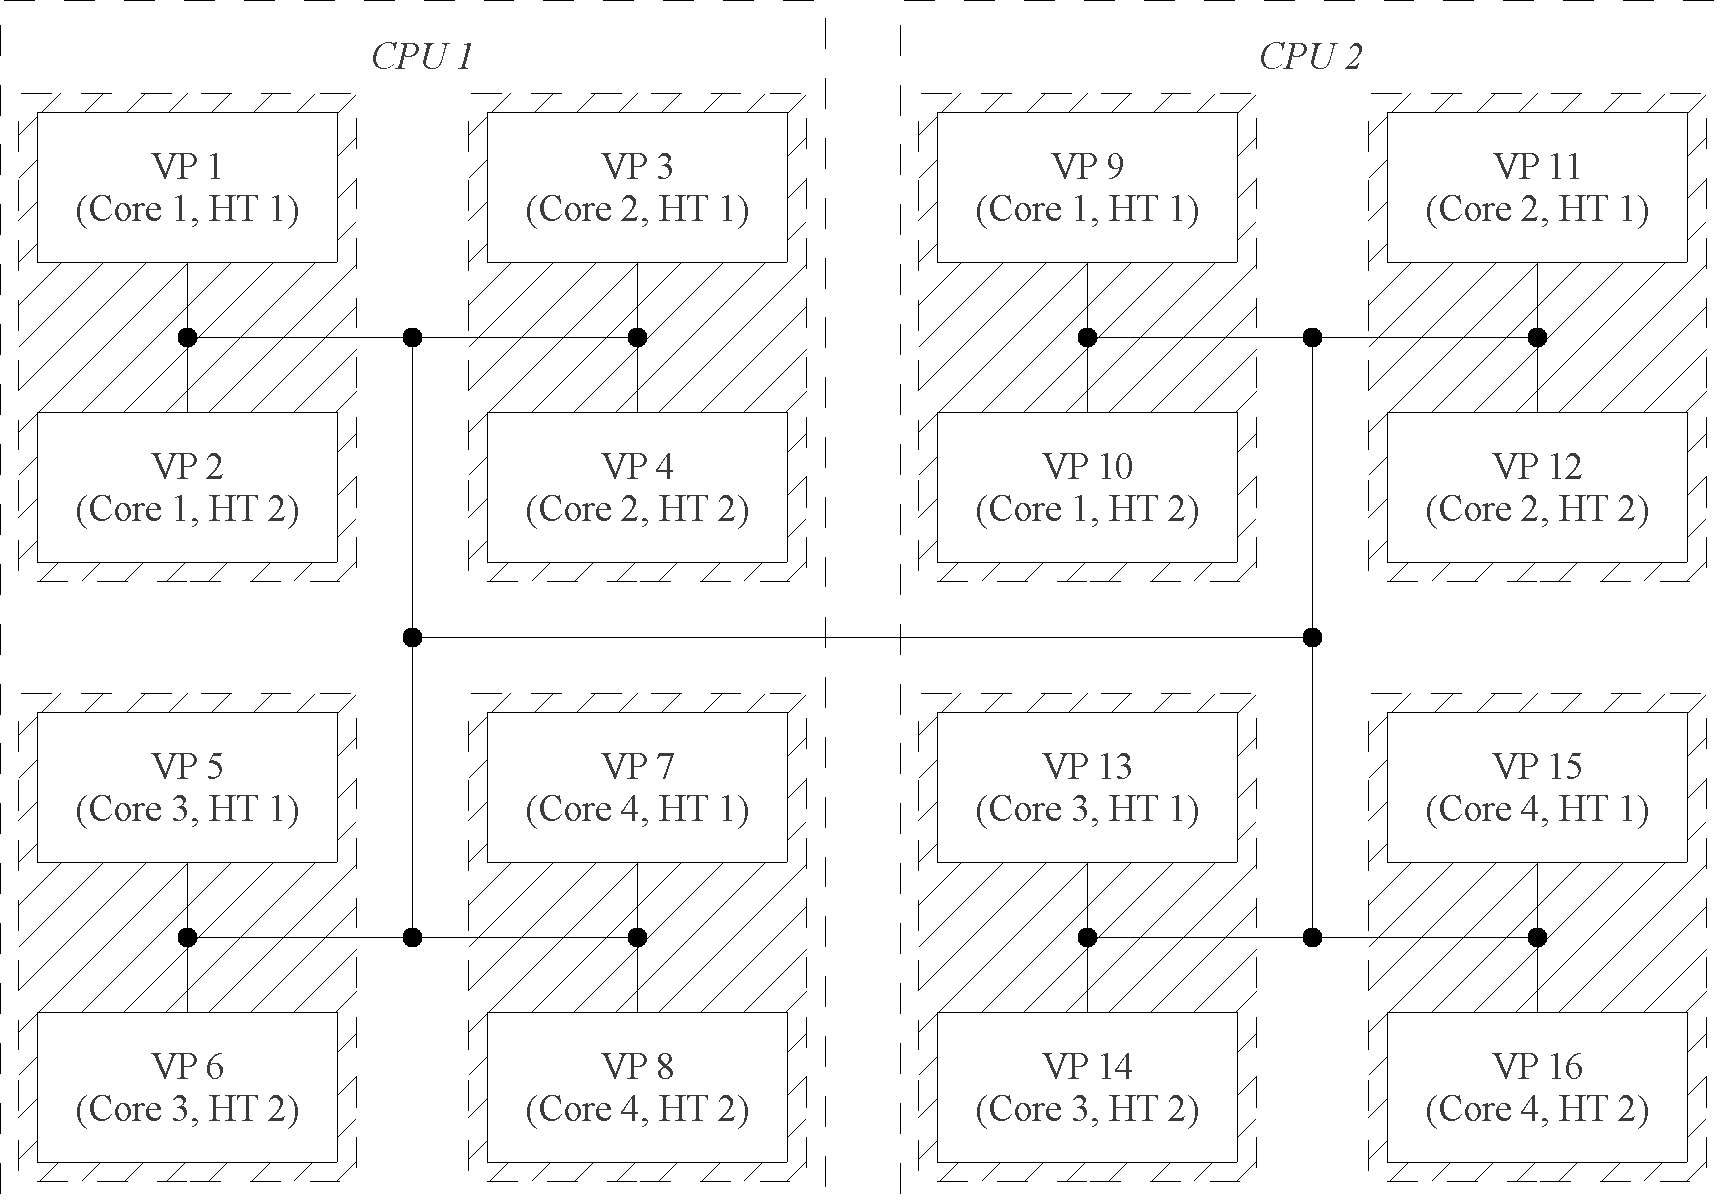
\includegraphics[width=12cm]{gfx/cpu_core_hyperthread_distances}
\caption[An example of how SALS allocates virtual processors for a
  hardware configuration with two multithreaded multicore
  processors.]{An example of how SALS allocates virtual processors
  (VP) for a hardware configuration with two multithreaded multicore
  processors, each having four cores and each core having two
  hyperthreads (HT).  Each hyperthread is organized into a binary tree
  structure that is used in order to calculate distances between
  hardware hyperthreads.  This binary tree distance metric is used to
  dynamically distribute fiber loads across hyperthreaded CPU cores in
  order to attempt to utilize as much on-chip CPU cache as possible.}
\label{figure:cpu_core_hyperthread_distances}
\end{figure}

The SALS virtual machine has been tested with a maximum of 32
processors and 128 gigabytes of RAM on the Nautilus supercomputer at
the National Institute for Computational Sciences.  However, most of
the examples presented in this dissertation have been executed on a
personal computer with only 4 CPU cores and 2 hyperthreads per core.
The SALS virtual machine has a tricolor garbage collection algorithm
that takes advantage of parallelizing work in concurrent processors.
Memory pointers in the SALS memory system are 64-bit integers that
have space reserved for three hierarchical memory tiers: (1)
``computer identity,'' (2) ``pool index,'' (3) and ``block address.''
{\mbox{\autoref{table:sals_memory_pointer}}} shows the bit allocation
within the 64-bit SALS memory pointer.
\begin{table}
\centering
\begin{tabular}{|l|l|l|}
\hline
\emph{bit range} &\emph{\# of values} &\emph{memory tier name} \\
\hline
~1 -- 17 &$131,072$         &computer identity \\ % 17
\hline
18 -- 27 &$1,024$           &pool index        \\ % 10
\hline
28 -- 64 &$137,438,953,472$ &block address     \\ % 37
\hline
\end{tabular}
\caption[Bit allocation within the SALS memory pointer.]{Bit
  allocation within the SALS memory pointer.}
\label{table:sals_memory_pointer}
\end{table}
The computer identity is zero if the memory pointer is referencing
memory on the local computer.  The computer identity is an integer
greater than zero if the memory is on another computer that has
connected to the SALS memory system through a low-level peer-to-peer
socket connection.  The ability of the SALS architecture to connect to
other running SALS architectures allows it to potentially scale to
take advantage of the hardware on multiple networked computers to
solve one large shared-memory problem.  The pool index is an integer
reference into an array of memory pools on the given computer.  On any
given computer, one memory pool is allocated for each hyperthread in
each CPU core on each CPU.  The block address is an integer that is a
block index into the given memory pool.  A block size of one byte has
been used for the examples presented in this dissertation but larger
block sizes have been tested and can be used if more memory must be
addressed.

\section{Package Manager}

The SALS programming language allows compiling and running computer
programs that consist of many thousands of lines of code.  For
example, the examples presented in this dissertation depend on loading
154 packages, which are composed of over 30,000 lines of code that are
written in the SALS low-level Lisp-like programming language.  The
SALS programming language includes a package manager in order to
organize dependencies within this codebase.  In addition to a
low-level Lisp-like codebase of packages, the SALS virtual machine has
the ability to load packages that contain optimized routines that are
composed of compiled machine code.  Machine code extensions to the
SALS virtual machine are written in the C programming language.  The C
codebase that compiles to this machine code totals over 150,000 lines
of C code.  The following is a declaration of a package definition in
the SALS low-level Lisp-like language that helps to organize these
different types of dependencies within the SALS codebase:
\begin{samepage}
\begin{Verbatim}
  [defpackage semantic_knowledge_base
    :packages          [equals_hash
                        forgetful_event_stream
                        semantic_realm
                        semantic_causal_event
                        semantic_relationship_key
                        semantic_frame
                        semantic_object
                        semantic_event]
    :sources           ['semantic_knowledge_base-core.sals']
    :dynamic_libraries ['libf2e_semantic_knowledge_base.so']]
\end{Verbatim}
\end{samepage}
The ``defpackage'' expression in the SALS programming language means
``define package.''  The first argument to the defpackage expression
is the name of the package to be defined, ``semantic knowledge base''
in this case.  The remaining arguments to the defpackage expression
are optional and three such arguments are shown in this example: (1)
``packages,'' (2) ``sources,'' and (3) ``dynamic libraries.''  The
``packages'' optional argument specifies a list of other packages that
must be loaded before this package is loaded.  The ``sources''
optional argument specifies a list of SALS low-level Lisp-like
programming language files that are to be loaded when this package is
loaded.  The ``dynamic libraries'' optional argument specifies a list
of files that contain machine code extensions that should be loaded
into the SALS virtual machine when this package is loaded.

Every package and machine code extension to the SALS virtual machine
and programming language performs ``causal reflective tracing'' on
each concurrently executing process.  The following sections describe
examples of different uses of the causal reflective tracing features
that have been implemented throughout the SALS virtual machine and its
extensions.  At the end of this chapter I will describe one high-level
package in the SALS programming language that performs the conjunctive
hypothesis space version space rule-learning algorithm, which is key
to the asynchronous experiential learning presented in
{\mbox{\autoref{chapter:learning_asynchronously_from_experience}}}.

\section{Causal Reflective Tracing}

Parallel tasks in the virtual machine are called ``fibers'' in order
to distinguish them from the ``threads'' in the underlying operating
system kernel.  The parallel fibers create, mutate, and read from
memory as they execute sequences of compiled bytecodes.  At any point
between bytecode executions, the memory system is static and can be
saved or loaded from non-volatile memory, such as a harddisk.  The
current execution state of every fiber is represented in the global
environment.  To be fully reflective on all of the procedural effects
of any given fiber, I introduce a technique called ``causal reflective
tracing.''  Causal reflective tracing is a way of defining variables
that are specific to each fiber that can be used to control the
low-level memory access, mutation, and creation functions.  This
allows one fiber to subscribe to the procedural trace events of
another fiber without receiving procedural trace events of its own
execution, which would lead to an infinite regress, halting the
system.  Further, because the virtual machine is inherently a parallel
processing system, a given fiber will often start a number of child
fibers that handle part of the processing for the parent fiber.  When
a new fiber is created, the child fiber inherits the causal variable
bindings of its parent fiber, enabling the same procedural tracing
options for the child as well.  So, causal reflective tracing is one
of the basic tools for keeping track of which pieces of memory were
created, mutated, or read by which other fibers.  When evaluating the
theoretical time complexity of concurrent procedurally reflective
control algorithms, it should be noted that creating procedural trace
events for the execution of a given fiber slows the fiber down only by
a constant factor, not affecting the algorithm's ``big-O'' time
complexity on an ideal concurrent shared-memory system, of which the
virtual machine is an approximation.

While causal reflective tracing focuses the procedural event tracing
to memory interactions of specific groups of fibers, this still
results in millions of events to consider every real-time second of
execution.  In order to further focus on specific objects within the
memory system, specific pieces of memory can be created called
``semantic memory.''  Semantic memory objects are created, mutated,
and accessed in roughly the same way as all of the frame-based objects
in the memory system with a few extra reflective tracing features.
For example, semantic objects provide event streams that can be
subscribed to by a number of different parallel listeners in different
fibers.  Also semantic object pointers are bidirectional in order to
ease traversal by reflective pattern matching algorithms.

Because it becomes awkward to subscribe to each and every frame-based
object that may be interesting to the reflective focus, semantic
frames that are created by specific fibers can be added to collections
of semantic frames that are called ``semantic knowledge bases.''
Semantic knowledge bases are good for organizing entire layers or
subsets of reflective layers that contain different types of semantic
frame objects.  Semantic knowledge bases allow the same forgetful
event stream subscription services as semantic frames with the
additional capability of tracing the addition and removal of entire
semantic frames to and from the knowledge base.

While knowledge base reconstructions are extremely fast to reference,
$O(1)$, they require a duplication of the memory requirements of the
focus knowledge base for every different point in time that is
required.  In order to allow efficient access of the state of
knowledge bases at arbitrary points in the past, ``semantic event
knowledge bases'' are another type of representation that is
reflectively and asynchronously maintained in order to not slow down
the primary procedure under reflective focus.
{\mbox{\autoref{chapter:learning_asynchronously_from_experience}}}
describes how the SALS asynchronous learning algorithm uses the event
knowledge base object to calculate partial state transframes.  I will
briefly review the features of the event knowledge base as well as a
few details about how this object is initialized and used in the SALS
low-level Lisp-like programming language.  The semantic event
knowledge base stores a type of semantic frame called a ``semantic
event.''  A semantic event is a type of semantic frame object that
represents an interval in time, which may include partial knowledge if
the start or end times do not exist, making the interval potentially
open-ended.  Semantic event knowledge bases are reflectively traced
and the knowledge is always stored in two different representations,
the basic semantic event frames as well as a balanced interval tree
that always represents the current state of the semantic event
knowledge base.  The balanced interval tree allows accessing the state
of the focus knowledge base in $O(\log{(n)})$ time, where $n$ is the
number of events stored in the semantic event knowledge base.
Although the time complexity is not as efficient as the constant,
$O(1)$, access time of the reflectively reconstructed semantic
knowledge base, the semantic event interval tree knowledge base only
requires $O(n)$ memory complexity in order to allow access to the
structure of the knowledge base at any point in the past, where $n$ is
the number of semantic events.
{\mbox{\autoref{figure:semantic_event_knowledge_base}}} shows how to
create a new ``{\tt{semantic\_event\_knowledge\_base}}'' type object
in the SALS low-level Lisp-like interactive programming language.
\begin{figure}[h]
\centering
{\scriptsize
\begin{Verbatim}[frame=single]
 in-> [new semantic_event_knowledge_base nil [new semantic_realm]]
out-> [semantic_event_knowledge_base
        semantic_event_tree         [semantic_event_tree ...]
        semantic_frame_set          [set ...]
        trace_remove_semantic_frame []
        trace_callback_funks_frame  [frame ...]
        semantic_realm              [semantic_realm ...]
        trace_event_stream          [forgetful_event_stream ...]
        trace_add_semantic_frame    []
        ...]
\end{Verbatim}
}
\caption[How to create a new
  ``{\tt{semantic\_event\_knowledge\_base}}'' type object.]{How to
  create a new ``{\tt{semantic\_event\_knowledge\_base}}'' type
  object.  When ``{\tt{semantic\_event}}'' type objects are added,
  removed, or modified while they are in this type of knowledge base,
  the knowledge base updates an always-accurate event interval tree
  structure for all of the events for efficient, $O(\log{(n)})$,
  access to the events at any point in time.}
\label{figure:semantic_event_knowledge_base}
\end{figure}

By default, when there are no listeners to the procedural event
streams of a semantic frame-based object, no reflective events are
created, allowing the use of the object to run at full speed.  When a
listener subscribes to the procedural use of a specific semantic
memory object, events are added to ordered streams for the listening
subscribers.  In order to conserve memory resources, when multiple
parallel listeners are subscribed to a given event stream, only those
events that have not already been seen by all of the subscribers are
remembered.  Once all subscribers have processed an event, all events
before this event are forgotten.  This type of memory conserving event
stream is referred to as a ``forgetful event stream.''  In this way
semantic frames report the addition and removal of slot values to
reflective forgetful event stream subscribers.  Once a knowledge base
is created and we have an ``important event stream iterator,'' we can
define a concurrent reflective fiber that processes the events
reflectively, after the real-time execution of the processes that
modify this knowledge base.
{\mbox{\autoref{figure:reflective_fiber}}} shows an example of how a
reflective fiber can be created to process a
{\tt{forgetful\_event\_stream}} generated by a
{\tt{semantic\_knowledge\_base}}, which includes a traced
{\tt{semantic\_planner}}.
\begin{figure}[h]
\centering
{\scriptsize
\begin{Verbatim}[frame=single]
 in-> [let* [[realm          [new semantic_realm]]
             [knowledge_base [new semantic_event_knowledge_base
                                  nil realm]]
             [iterator       [get knowledge_base
                                  new-event_stream_iterator]]
             [planner        [new semantic_planner realm]]]

        'Start parallel reflective fiber.'
        [fiber [funk []
                 [while t
                   [let [[event [have iterator wait_for_current]]]
                     [print event]
                     [have iterator increment]]]]
               []]
        
        [set planner trace_add    t]
        [set planner trace_remove t]
        
        [have knowledge_base add_semantic_frame planner]
        
        [set planner imagine_time [new semantic_time [time]]]]
out-> []
\end{Verbatim}
}
\caption[A reflective fiber can be created to process an
  {\tt{forgetful\_event\_stream}}.]{A reflective fiber can be created
  to process a {\tt{forgetful\_event\_stream}} generated by a
  {\tt{semantic\_knowledge\_base}}, which includes a traced
  {\tt{semantic\_planner}}.  Note that this example runs at a constant
  factor slower than full speed because of the creation of mutation
  events for the {\tt{semantic\_planner}} object, but this factor has
  been kept relatively small, so this example completes almost
  immediately.  The reflective process runs slower because it must
  consider how to print these events to the terminal in a readable
  form.  {\mbox{\autoref{figure:remove_add_set_events}}} shows the
  last two events created by the last line of this example that
  mutates the {\tt{imagine\_time}} slot value for the planner.}
\label{figure:reflective_fiber}
\end{figure}

\begin{figure}[h]
\centering
{\scriptsize
\begin{Verbatim}[frame=single]
[semantic_frame_event
  time           [time
                   years        2012
                   months       8
                   days         31
                   ...]
  event_type     remove
  semantic_frame [semantic_planner
                   property phenomenal_name [...]
                   property planner_type    [[]]
                   property imagine_time    [[semantic_time ...]]
                   relation execute_plan    [[]]
                   relation imagine_plan    [[]]
                   relation focus_plan      [[]]
                   ...]
  key_type       property
  key            imagine_time
  value          []]
\end{Verbatim}
\begin{Verbatim}[frame=single]
[semantic_frame_event
  time           [time years 2012 months 8 days 31 hours 23 ...]
  event_type     add
  semantic_frame [semantic_planner
                   property phenomenal_name [...]
                   property planner_type    [...]
                   property imagine_time    [...]
                   relation execute_plan    [...]
                   ...]
  key_type       property
  key            imagine_time
  value          [semantic_time
                   value [time
                           years        2012
                           months       8
                           days         31
                           ...]]]
\end{Verbatim}
}
\caption[The last two events created by the last line of the example
  in {\mbox{\autoref{figure:reflective_fiber}}}.]{The last two events
  created by the last line of the example in
  {\mbox{\autoref{figure:reflective_fiber}}}:
  ``{\tt{[set~planner~imagine\_time~[new~semantic\_time~[time]]]}}''. This
  command mutates the {\tt{imagine\_time}} slot value for the planner.
  Notice that the first of the two events is a {\tt{remove}} type of
  event, while the second is an {\tt{add}} type event.  This event
  knowledge is used in the SALS AI to create reconstructions of entire
  knowledge bases of physical as well as deliberative object types,
  like planners.  Note that the first event removes the {\tt{[]}} slot
  value of the {\tt{imagine\_time}} {\tt{property}} of the
  {\tt{semantic\_planner}} object, while the second event adds the new
  value, thus completing the mutation.}
\label{figure:remove_add_set_events}
\end{figure}

While every parallel fiber is allocated a unique {\tt{cause}} object
that provides a representation of the reflective tracing features for
that fiber, sometimes it is useful to collect events from overlapping
sets or different hierarchies of many fiber objects.  A convenient
solution to causally organizing very dynamic sets of fibers is
provided by a ``cause group'' object.  Cause groups are added to cause
objects and inherited from parent to child when new causes are
created.  Because cause objects and cause group objects exist at the
locus of every memory creation and mutation event in the SALS virtual
machine, they provide a means of tracing any event that modifies any
part of the SALS virtual machine.
{\mbox{\autoref{figure:cause_group_statistics}}} shows an example of
causal reflective tracing that takes advantage of cause group objects
in order to gather run-time statistics of a fiber execution.
{\mbox{\autoref{figure:hierarchical_cause_group_statistics}}} shows
another example of using a hierarchy of multiple cause group objects
in order to causally scope the tracing of $30$ parallel fibers that
are hierarchically organized into $3$ cause groups that contain $10$
fibers each.
\begin{figure}[h]
\centering
{\scriptsize
\begin{Verbatim}[frame=single]
 in-> [globalize cause_group [new cause_group]]
out-> []

 in-> [with-new-cause
        [have [this-cause] add_cause_group cause_group]
        [partimes [i 10]
          [print i]]]
0
1
2
3
4
6
7

58
9
out-> []

 in-> cause_group
out-> [cause_group
        execution_nanoseconds 533248657
        bytes_allocated_count 2766181
        bytecode_count        19495
        bytes_freed_count     0]
\end{Verbatim}
}
\caption[Using a {\tt{cause\_group}} object to gather statistics from
  causally scoped executions.]{Using a {\tt{cause\_group}} object to
  gather statistics from causally scoped executions.  A new
  {\tt{cause\_group}} object is first created in the global
  environment.  The gathering of run-time statistics involves creating
  a new cause with the ``{\tt{with-new-cause}}'' operator, adding this
  cause to the {\tt{cause\_group}} object, and subsequently running an
  experiment.  This example creates ten parallel fibers that each
  print their numerical index from $0$ to $9$.  At the final output of
  the example, the global {\tt{cause\_group}} object is printed to the
  screen, showing processor execution time, total bytes allocated,
  total bytecodes executed, and also the number of bytes garbage
  collected during the experiment.}
\label{figure:cause_group_statistics}
\end{figure}
\begin{figure}[h]
\centering
{\scriptsize
\begin{Verbatim}[frame=single]
 in-> [globalize cause_group [new cause_group]]
out-> []

 in-> [let [[begin_time [time]]
            [frame      [new frame]]]
        [with-new-cause
          [have [this-cause] add_cause_group cause_group]
          [partimes [i 3]
            [let [[subcause_group [new cause_group]]]
              [have frame add i subcause_group]
              [with-new-cause
                [have [this-cause] add_cause_group subcause_group]
                [partimes [j 10]
                  [terminal_format standard-terminal j]]]]]]
        [have frame add `real-time [- [time] begin_time]]
        frame]
024031548162062794915695337878                      
out-> [frame
        0         [cause_group
                    execution_nanoseconds 3535418608
                    bytes_allocated_count 7715763
                    ...]
        2         [cause_group
                    execution_nanoseconds 3012761500
                    bytes_allocated_count 7590735
                    ...]
        1         [cause_group
                    execution_nanoseconds 3976116760
                    bytes_allocated_count 9598095
                    ...]
        real-time [relative_time
                    seconds      1
                    milliseconds 694
                    ...]]

 in-> cause_group
out-> [cause_group
        execution_nanoseconds 10730429054
        bytes_allocated_count 25622218
        bytecode_count        215649
        bytes_freed_count     0]
\end{Verbatim}
}
\caption[Gathering run-time statistics using parallel hierarchies of
  causal scopes.]{Gathering run-time statistics using parallel
  hierarchies of causal scopes.  Overall, $30$ parallel fibers are
  created, each prints a number from $0$ to $9$, and run-time
  statistics are gathered in two layers of causal scope hierarchy.
  The overall {\tt{cause\_group}} object is shown last, while three
  sub-{\tt{cause\_group}} objects are printed as the return value of
  the second expression.  Notice that the algorithm uses $10.7$
  seconds of processor time, while only using $1.7$ seconds of
  real-time.}
\label{figure:hierarchical_cause_group_statistics}
\end{figure}

Sometimes it is helpful to know which fiber or cause created a
specific piece of memory.  For this reason, every piece of memory in
the entire virtual machine includes a reference to its creation cause
as well as its creation fiber.
{\mbox{\autoref{figure:reflective_event_causal_tracing}}} shows how a
fiber can retrieve the creation cause of a semantic event object, it
is useful to know which fiber or cause is responsible for creating a
given semantic event object so that a reflective fiber can learn from
the separate effects of different causal scopes that make
modifications to semantic objects within a given knowledge base.  This
form of causal tracing is used in the SALS cognitive architecture to
detect when one resource interacts with another resource, for example,
by activating that resource or waiting for that resource to complete
execution.  An entire reflective knowledge base of current parallel
resource interactions is maintained by tracing the causes of resource
interactions in this way.
\begin{figure}[h]
\centering
{\scriptsize
\begin{Verbatim}[frame=single]
 in-> [let* [[realm          [new semantic_realm]]
             [knowledge_base [new semantic_event_knowledge_base
                                  nil realm]]
             [iterator       [get knowledge_base
                                  new-event_stream_iterator]]
             [planner        [new semantic_planner realm]]]

        'Start parallel reflective fiber.'
        [fiber [funk []
                 [while t
                   [let* [[event       [have iterator
                                             wait_for_current]]
                          [event-cause [get event cause]]]
                     [if [eq `my-test [have event-cause lookup
                                            `cause-name]]
                         [print `event-in-causal-focus]
                       [print `event-out-of-causal-focus]]
                     [have iterator increment]]]]
               []]
        
        [set planner trace_add    t]
        [set planner trace_remove t]
        
        [have knowledge_base add_semantic_frame planner]
        
        [with-new-cause
          [cause-define cause-name `my-test]
          [set planner imagine_time [new semantic_time [time]]]]]
out-> []
event-out-of-causal-focus
event-out-of-causal-focus
event-out-of-causal-focus
event-out-of-causal-focus
event-out-of-causal-focus
event-out-of-causal-focus
event-out-of-causal-focus
event-out-of-causal-focus
event-in-causal-focus
event-in-causal-focus
\end{Verbatim}
}
\caption[Causally scoped reflective event tracing.]{Causally scoped
  reflective event tracing.  Since every piece of memory in the
  virtual machine has a reference to its {\tt{cause}} object, causally
  focusing the reflective tracing example shown in
  {\mbox{\autoref{figure:reflective_fiber}}} is simply a matter of
  accessing the creation cause of each event, using the expression,
  {\tt{[get event cause]}}.}
\label{figure:reflective_event_causal_tracing}
\end{figure}

\section{Conjunctive Hypothesis Version Space Rule-Learning}

The SALS architecture includes a ``version space''
\cite[]{mitchell:1997} hypothesis rule-learning algorithm.  A use of
this hypothesis version space rule-learning algorithm was described in
{\mbox{\autoref{chapter:learning_asynchronously_from_experience}}} as
part of a larger asynchronous learning algorithm that learns to
predict the partial state ``transframe'' \cite[]{minsky:1975} effects
of resource executions given the partial state preconditions of the
execution.  The hypothesis version space rule-learning algorithm
included in the SALS architecture predicts one binary output feature
given a number of binary input features.  The benefit of the version
space rule-learning algorithm is that it provides a relatively compact
representation of an entire conjunctive hypothesis space by only
representing the most general and most specific boundaries in the
overall lattice of potential hypotheses.  The included rule-learning
algorithm is incremental, meaning that it refines its space of
hypotheses as new examples of training data become known.  The SALS AI
hypothesis version space learning algorithm also includes ``removal
callbacks'' for most general and most specific hypotheses, so that if
these hypotheses are no longer supported given new training data,
these hooks allow tracing dependencies for correcting hypothetically
supported counterfactual knowledge in the counterfactual knowledge
base of each planning layer of the SALS AI.
{\mbox{\autoref{figure:concept_version_space}}} shows how to create a
{\tt{concept\_version\_space}} object that can be trained.
{\mbox{\autoref{figure:concept_version_space_training}}} shows an
example of training the {\tt{concept\_version\_space}} object, given
training examples.
{\mbox{\autoref{figure:concept_version_space_hypothetical_support}}}
shows how hypothesis removal callbacks can be used to monitor the loss
of support for a specific example, attempting to find new support
whenever the previous hypothetical support is lost.
\begin{figure}[h]
\centering
{\scriptsize
\begin{Verbatim}[frame=single]
 in-> [new concept_version_space]

out-> [concept_version_space
        specific_hypotheses [[concept_version_space_hypothesis]]
        general_hypotheses  [[concept_version_space_hypothesis]]
        variable_name_set   [set elements []]]
\end{Verbatim}
}
\caption[Creating a new {\tt{concept\_version\_space}} conjunctive
  hypothesis learning algorithm.]{Creating a new
  {\tt{concept\_version\_space}} conjunctive hypothesis learning
  algorithm.  This object keeps a list of the most specific hypotheses
  that support positive output predictions as well as the most general
  hypotheses that support negative output predictions.  Also, there is
  a set of variable names, or frame slot names, that the algorithm has
  seen previously.}
\label{figure:concept_version_space}
\end{figure}
\begin{figure}[h]
\centering
{\scriptsize
\begin{Verbatim}[frame=single]
 in-> [let [[concept [new concept_version_space]]]
   
        'Add a positive training example to the concept.'
        [let [[example [new concept_version_space_example t]]]
          [have example add_variable_value `color `blue]
          [have example add_variable_value `shape `cube]
          [have concept train_on_example example]]

        [terminal_format standard-terminal
                         '\ntrain-1: ' concept]
        
        'Add a negative training example to the concept.'
        [let [[example [new concept_version_space_example nil]]]
          [have example add_variable_value `color `blue]
          [have example add_variable_value `shape `pyramid]
          [have concept train_on_example example]]
        
        concept]
train-1: [concept_version_space
           specific_hypotheses [[concept_version_space_hypothesis
                                  shape cube
                                  color blue]]
           general_hypotheses  [[concept_version_space_hypothesis
                                  shape ?
                                  color ?]]]
out-> [concept_version_space
        specific_hypotheses [[concept_version_space_hypothesis
                               shape cube
                               color blue]]
        general_hypotheses  [[concept_version_space_hypothesis
                               shape cube
                               color ?]]]
\end{Verbatim}
}
\caption[Training a {\tt{concept\_version\_space}} conjunctive
  hypothesis learning algorithm.]{Training a
  {\tt{concept\_version\_space}} conjunctive hypothesis learning
  algorithm.  A new {\tt{concept\_version\_space}} is created.  Two
  {\tt{concept\_version\_space\_example}}s are created, one positive
  and one negative.  The concept is printed after learning from the
  positive example.  The final concept is returned after being trained
  on both examples.}
\label{figure:concept_version_space_training}
\end{figure}
\begin{figure}[h]
\centering
{\scriptsize
\begin{Verbatim}[frame=single]
 in-> [let [[concept [new concept_version_space]]]
        [print 'Training on positive example.']
        [let [[example [new concept_version_space_example t]]]
          [have example add_variable_value `color `blue]
          [have example add_variable_value `shape `cube]
          [have concept train_on_example example]]
        [print 'Adding removal callbacks to hypotheses.']
        [let [[example [new concept_version_space_example t]]]
          [have example add_variable_value `color `green]
          [have example add_variable_value `shape `cube]
          [label find_new_support []
            [mapc [funk [hypothesis]
                    [terminal_format standard-terminal
                                     '\nNew supporting '
                                     'hypothesis: ' hypothesis]
                    [have hypothesis add_removal_callback
                                     [funk []
                                       [print 'Lost support.']
                                       [find_new_support]]
                                     []]]
                  [get concept supporting_hypotheses example]]]
          [find_new_support]]
        [print 'Training on negative example.']
        [let [[example [new concept_version_space_example nil]]]
          [have example add_variable_value `color `blue]
          [have example add_variable_value `shape `pyramid]
          [have concept train_on_example example]]
        [print 'Done.']
        nil]
'Training on positive example.'
'Adding removal callbacks to hypotheses.'
New supporting hypothesis: [concept_version_space_hypothesis
                             shape ?
                             color ?]
'Training on negative example.'
'Lost support.'
New supporting hypothesis: [concept_version_space_hypothesis
                             shape cube
                             color ?]
'Done.'
out-> []
\end{Verbatim}
}
\caption[Hypothesis removal callbacks used to monitor the loss of
  support for a specific example, attempting to find new support
  whenever the previous hypothetical support is lost.]{Hypothesis
  removal callbacks monitor the loss of support for a specific
  example, attempting to find new support whenever the previous
  hypothetical support is lost.  In this case, a positive example of a
  {\tt{green}} {\tt{cube}} is attempting to maintain hypothetical
  support in the concept's hypothesis space.}
\label{figure:concept_version_space_hypothetical_support}
\end{figure}


